% !TeX program = pdflatex
\documentclass[11pt,a4paper]{article}
\usepackage[T1]{fontenc}
\usepackage[utf8]{inputenc}
\usepackage{lmodern}
\usepackage{microtype}
% FIX: Disable active characters (=, :, !) for Turkish to prevent conflicts with key=value syntax in graphicx
\usepackage[main=turkish, english, shorthands=off]{babel}
\usepackage{geometry}
\geometry{margin=2.5cm}
\usepackage{graphicx}
\usepackage{booktabs}
\usepackage{array}
\usepackage{tabularx}
\usepackage{siunitx}
\sisetup{group-separator = {\,}, output-decimal-marker = {.}}
\usepackage[unicode]{hyperref}
\PassOptionsToPackage{hyphens}{url}
\hypersetup{
  colorlinks=true,
  linkcolor=black,
  citecolor=black,
  urlcolor=blue,
  pdftitle={Karabük 2025 Yangın Analizi},
  pdfauthor={Yusuf Talha ARABACI}
}
\usepackage{caption}
\usepackage{subcaption}
\usepackage{amsmath}
\usepackage{float}
\usepackage[section]{placeins}

\title{Karabük 2025 Orman Yangınları Görüntü İşleme Analizi}
\author{Yusuf Talha ARABACI\\Karabük Üniversitesi\\ Yazılım Mühendisliği Yüksek Lisans Öğrencisi}
\date{Aralık 2025}

% Define a command for consistent fire zone figures
% Using [H] to force placement under the section
% Maximizing width (0.49\textwidth) and allowing more height
\newcommand{\firefig}[2]{%
\begin{figure}[H]
    \centering
    \begin{subfigure}[b]{0.49\textwidth}
        \centering
        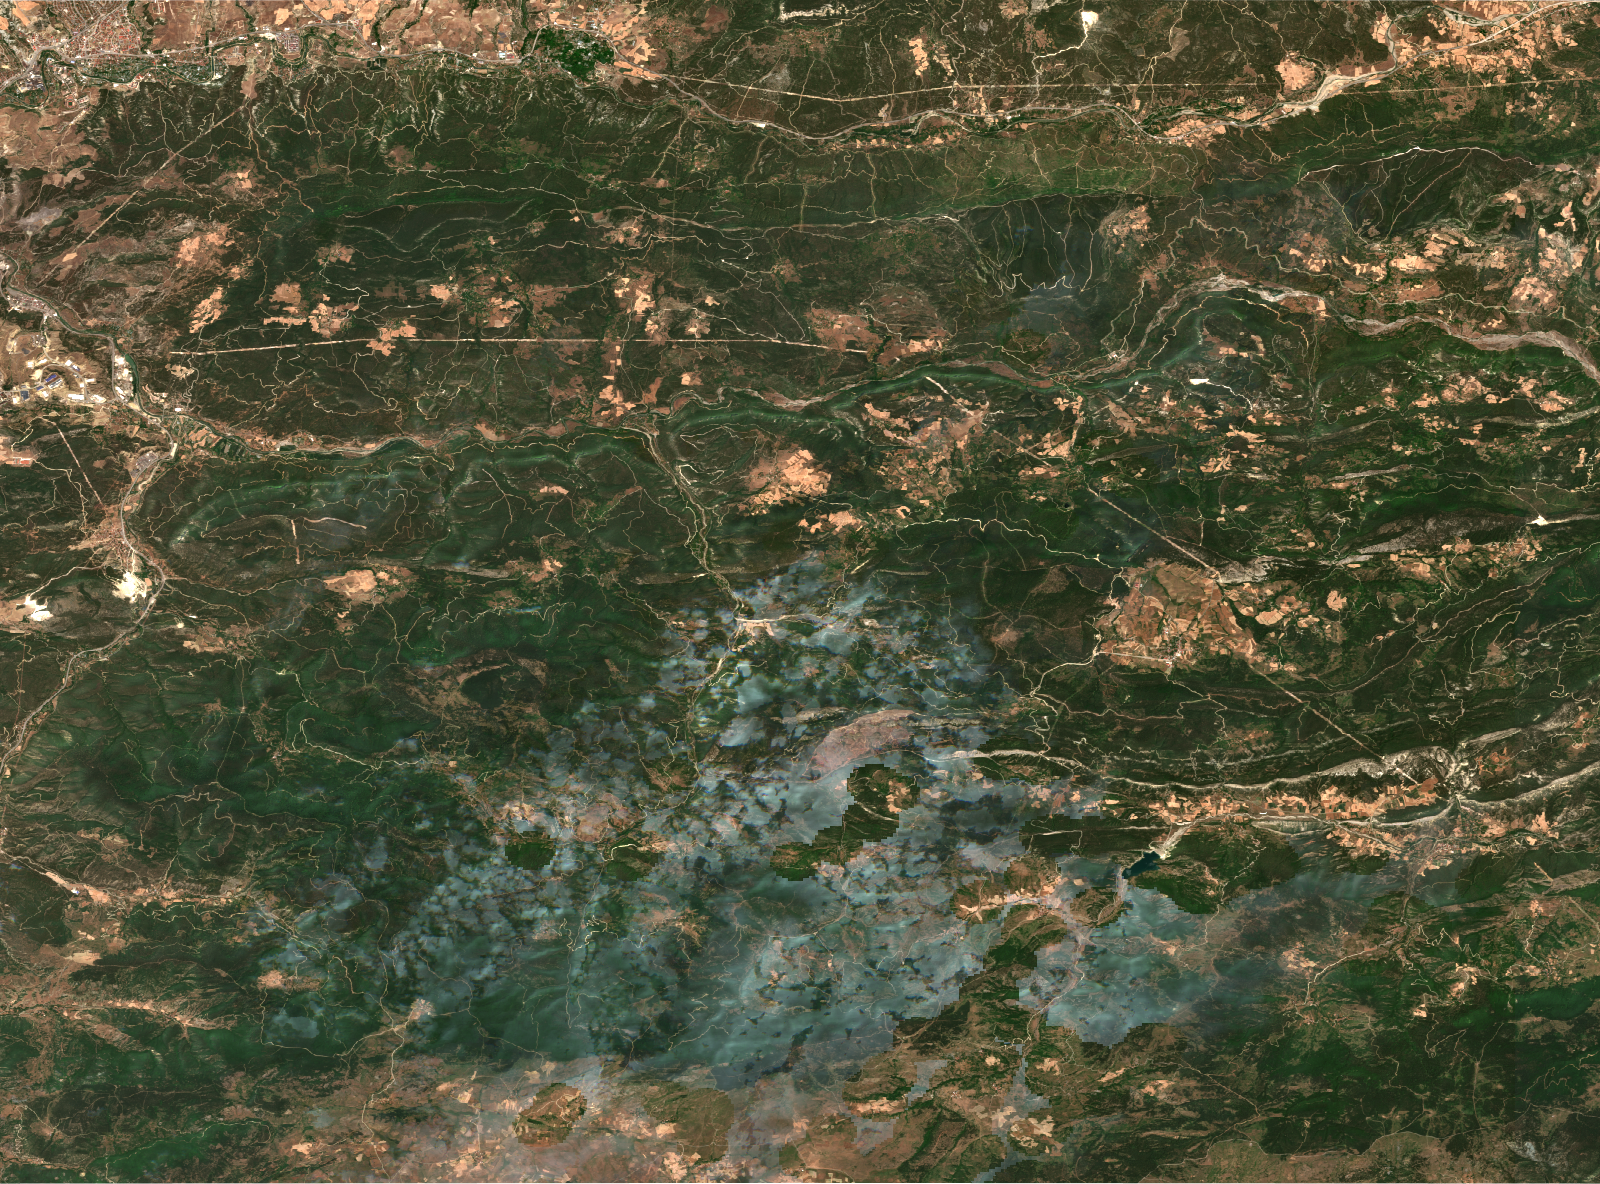
\includegraphics[width=\textwidth,height=0.28\textheight,keepaspectratio]{#1/pre_RGB.png}
        \caption{Öncesi}
    \end{subfigure}
    \hfill
    \begin{subfigure}[b]{0.49\textwidth}
        \centering
        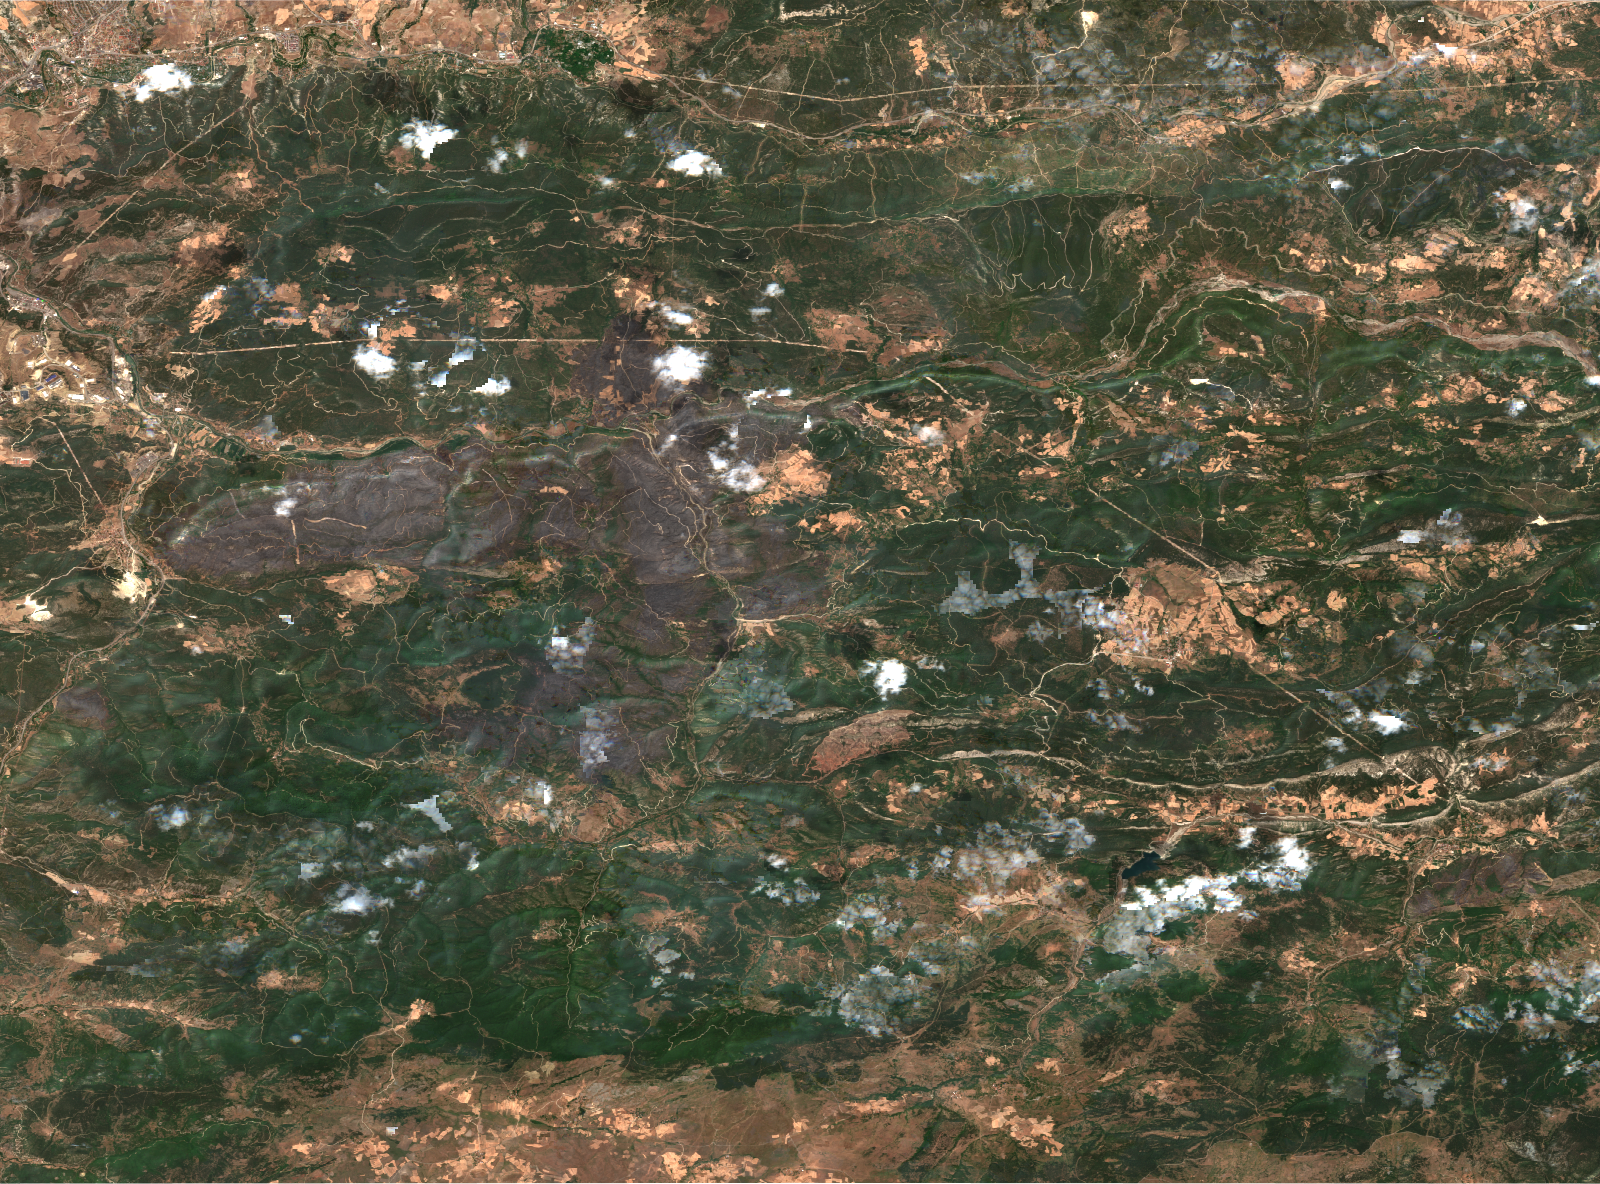
\includegraphics[width=\textwidth,height=0.28\textheight,keepaspectratio]{#1/post_RGB.png}
        \caption{Sonrası}
    \end{subfigure}
    \par\medskip
    \begin{subfigure}[b]{0.49\textwidth}
        \centering
        \includegraphics[width=\textwidth,height=0.28\textheight,keepaspectratio]{#1/dNDVI.png}
        \caption{dNDVI}
    \end{subfigure}
    \hfill
    \begin{subfigure}[b]{0.49\textwidth}
        \centering
        \includegraphics[width=\textwidth,height=0.28\textheight,keepaspectratio]{#1/dNBR.png}
        \caption{dNBR}
    \end{subfigure}
    \caption{#2}
\end{figure}
}

\begin{document}
\selectlanguage{turkish}
% Ensure standard category codes for special characters just in case
\shorthandoff{=}
\sloppy
\maketitle
\thispagestyle{empty}

\begin{abstract}
Bu proje, 2025 yaz sezonunda Karabük ilinde (özellikle Ovacık, Safranbolu ve Eflani bölgelerinde) meydana gelen orman yangınlarının çevresel etkilerini \textbf{sayısal görüntü işleme teknikleriyle} analiz etmek için geliştirilmiştir. 
\textbf{Google Earth Engine (GEE) Python API} kullanılarak yangın öncesi ve sonrası uydu görüntüleri işlenmiştir. Hasar tespitinde \textbf{temel metrik olarak dNBR (Normalized Burn Ratio Difference)} algoritması kullanılırken, bitki örtüsü değişimini doğrulamak amacıyla \textbf{dNDVI} verilerinden de yararlanılmıştır. 
Çalışma, geleneksel haber takibinin ötesine geçerek, yangın izlerini piksel tabanlı matematiksel modellerle doğrulamayı ve mühendislik yaklaşımıyla raporlamayı hedefler.
\end{abstract}

% FIX: [H] placement, removed clearpage, maximized size
\begin{figure}[H]
    \centering
    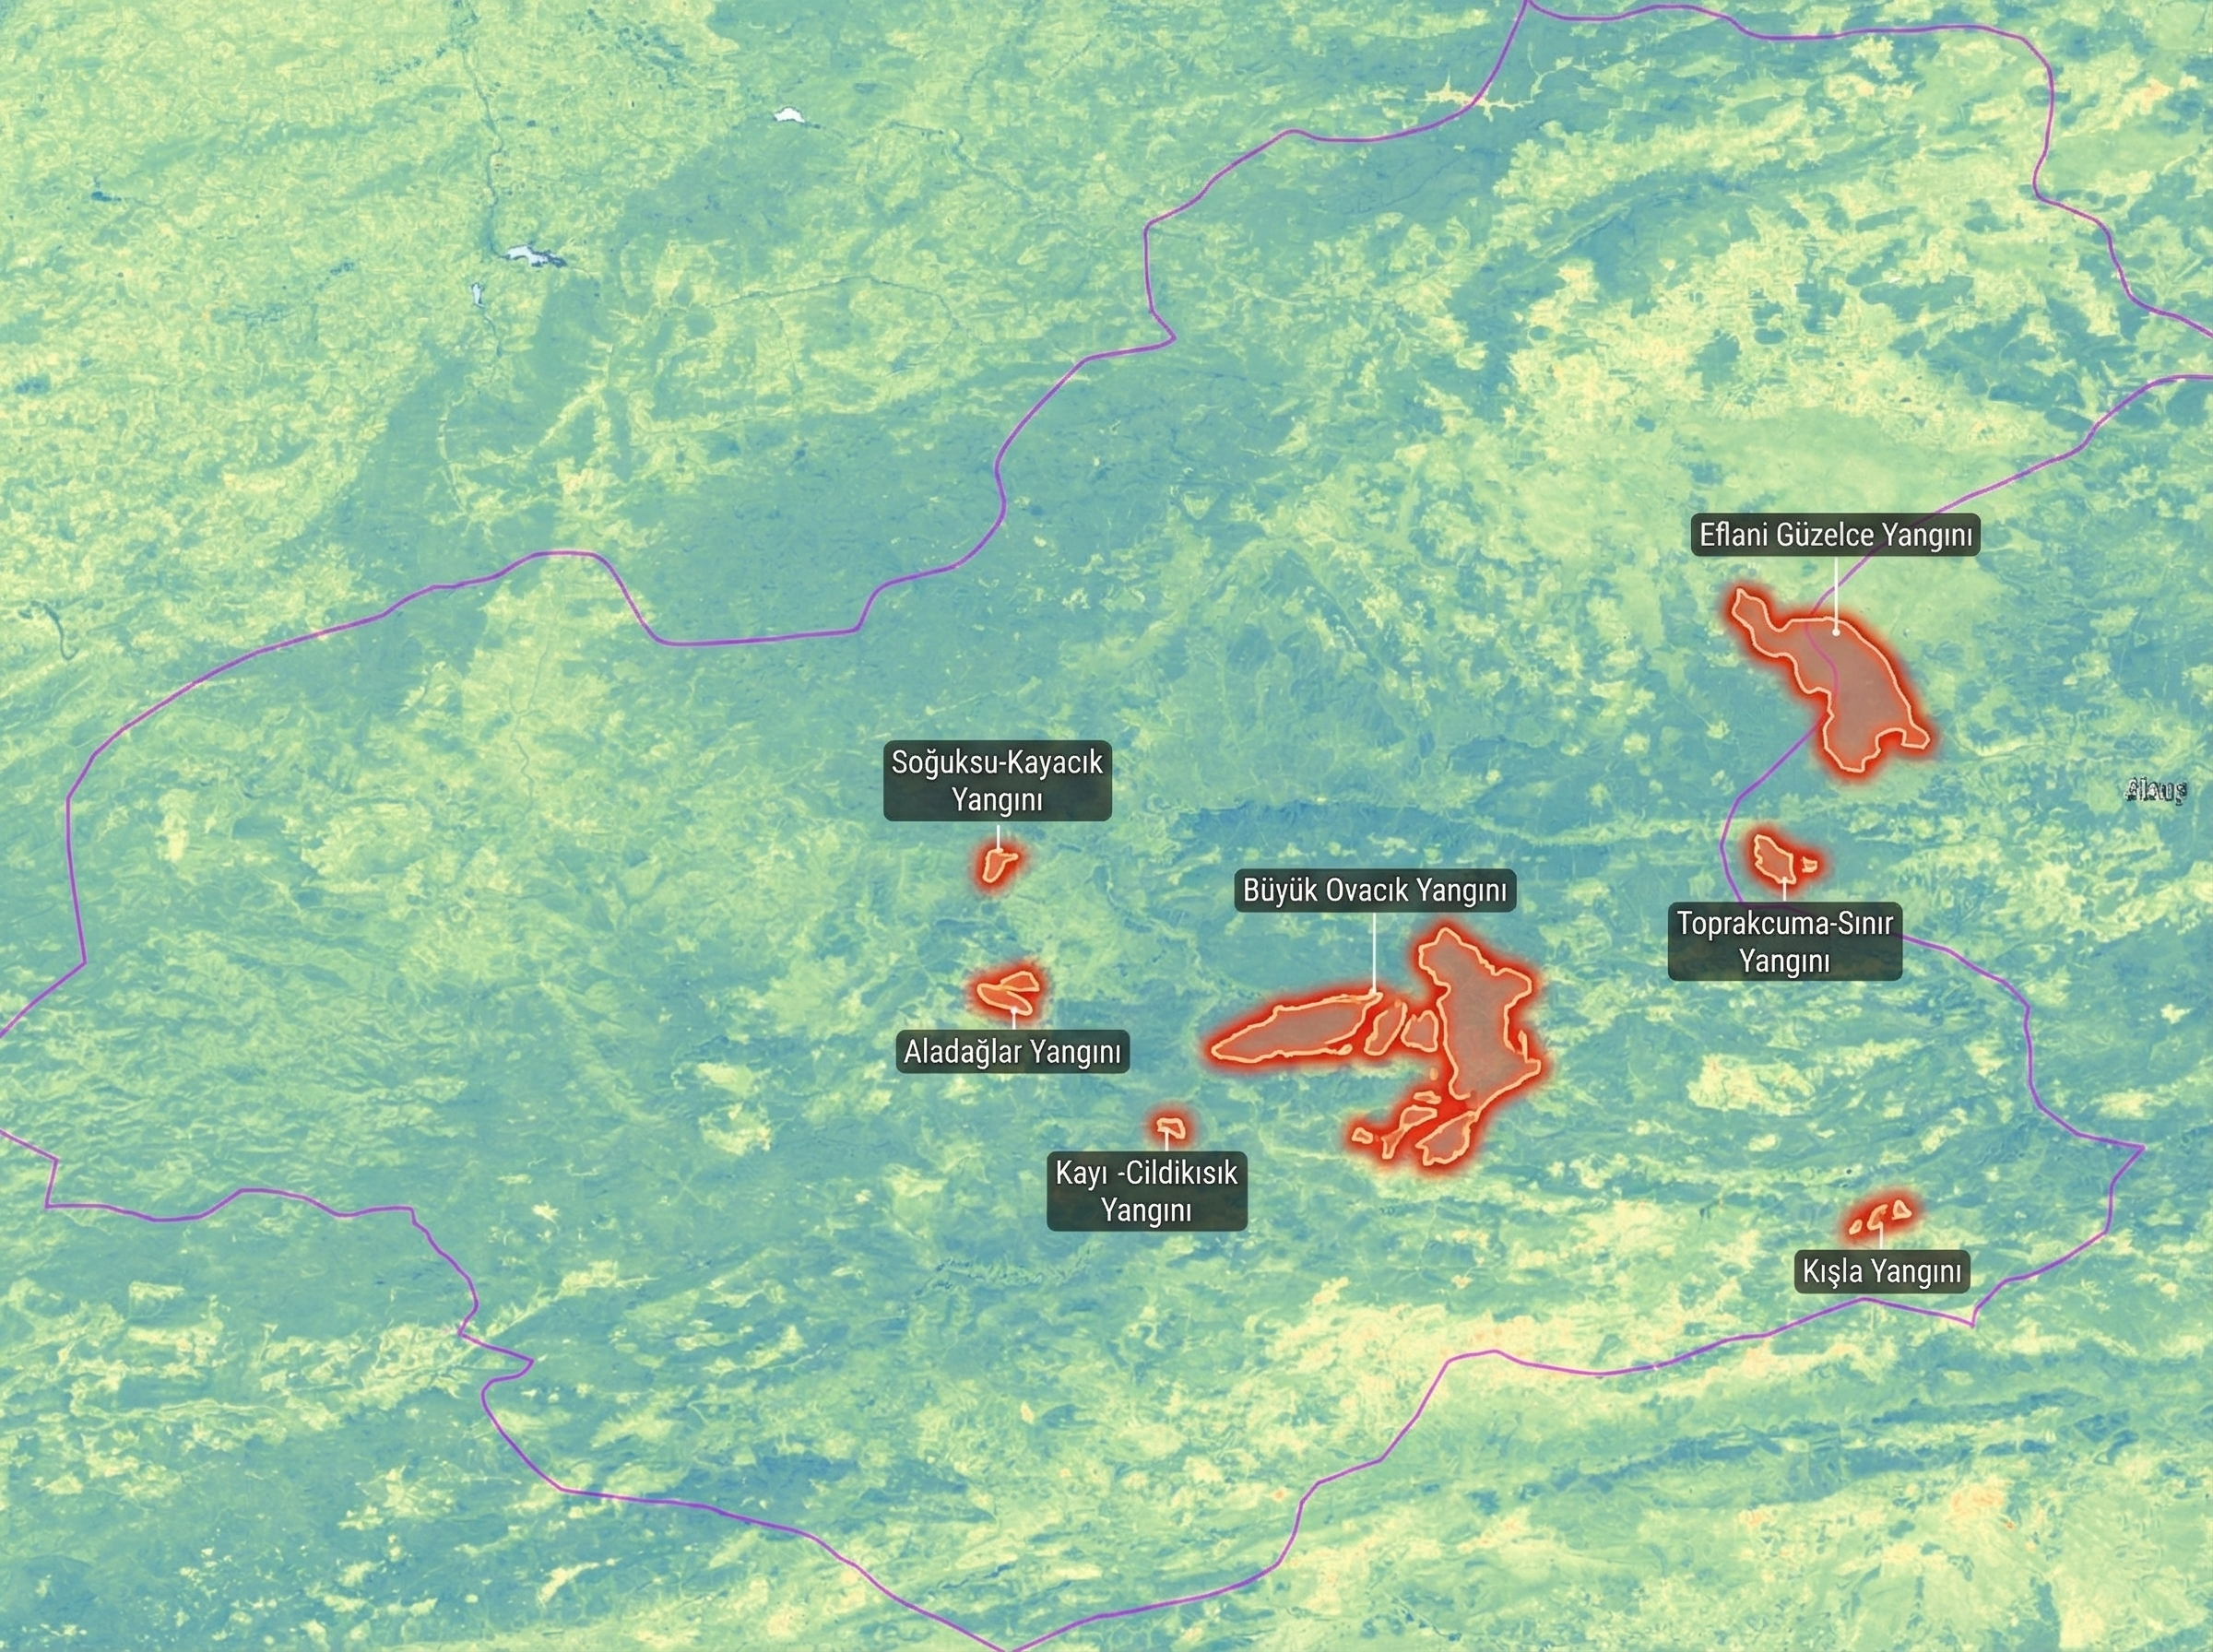
\includegraphics[width=1.0\textwidth,height=0.45\textheight,keepaspectratio]{figures/overview.png}
    \caption{Sentinel-2 Verileri ile Elde Edilen Karabük İli Geneli Yangın Dağılım Haritası}
    \label{fig:overview}
\end{figure}

\clearpage


\section{Giriş}
Sayısal görüntü işleme teknikleri, afet yönetimi ve çevresel izleme süreçlerinde ham uydu verilerinin anlamlı bilgiye dönüştürülmesinde kritik rol oynamaktadır. Bu çalışmada, Karabük ilindeki orman yangınları ele alınmıştır. Yüzölçümünün \%65'ini ormanların oluşturduğu Karabük ili, özellikle karaçam ve göknar ağırlıklı bitki örtüsüyle yangın hassasiyeti yüksek bir bölgedir. 2025 sezonunda bu durumdan önemli ölçüde etkilenmiştir. Özellikle Temmuz ve Eylül aylarında yoğunlaşan atmosferik koşullar (yüksek sıcaklık, düşük nem ve şiddetli rüzgar), il genelinde büyük ölçekli yangınları tetiklemiş, resmi makamlarca yapılan açıklamalara göre 36 farklı olayda toplam 6.865 hektar alanın zarar gördüğü bildirilmiştir. Bu çalışma, Sentinel-2 optik uydu verilerini kullanarak, devletin resmi kanalları ve basın yoluyla duyurulan bu yangınların etki alanını görselleştirmeyi ve mekansal dağılımını haritalamayı amaçlamaktadır. Analiz, resmi veriler ışığında uydu tabanlı yanma şiddeti (burn severity) sınıflaması ile saha gerçekleri arasındaki ilişkiyi irdelemektedir.

\section{Materyal ve Yöntem}
Bu çalışmada, Google Earth Engine (GEE) platformu üzerinde Python API kullanılarak piksel tabanlı görüntü işleme akışı (pipeline) geliştirilmiştir. Metodoloji; veri ön işleme, maskeleme, spektral indeks hesaplama ve eşik tabanlı sınıflandırma (thresholding) olmak üzere dört ana aşamadan oluşmaktadır.

\subsection{Veri Seti ve Ön İşleme}
Analiz için Avrupa Uzay Ajansı'nın (ESA) \textbf{Sentinel-2 MSI} (MultiSpectral Instrument) sensöründen elde edilen \textbf{Level-2A} (Atmosferik düzeltmesi yapılmış) yüzey yansıma verileri kullanılmıştır.

\begin{itemize}
    \item \textbf{Veri Koleksiyonu:} \texttt{COPERNICUS/S2\_SR\_HARMONIZED}
    \item \textbf{Zamansal Filtreleme:}
    \begin{itemize}
        \item \textit{Yangın Öncesi:} 1 Temmuz 2025 -- 20 Temmuz 2025
        \item \textit{Yangın Sonrası:} 5 Eylül 2025 -- 30 Eylül 2025
    \end{itemize}
\end{itemize}

\subsection{Maskeleme Algoritmaları}
Görüntü üzerindeki gürültüyü (noise) temizlemek ve analizi sadece ilgili alanlara odaklamak için iki aşamalı maskeleme uygulanmıştır:

\begin{enumerate}
    \item \textbf{Bulut ve Sirüs Maskeleme (QA60 Bitmask):} Sentinel-2 verisindeki \texttt{QA60} bandı kullanılarak bulutlu ve sirüs (cirrus) bulutu içeren pikseler maskelenmiştir. Bit 10 (opak bulutlar) ve Bit 11 (sirüs bulutları) 0'a eşit olmayan pikseller analiz dışı bırakılmıştır.
    \item \textbf{Arazi Örtüsü Maskeleme:} Yanmış alanların tarım arazisi hasadı veya şehirleşme ile karışmasını önlemek amacıyla \textbf{ESA WorldCover v100} veri seti kullanılmıştır. Sadece aşağıdaki sınıflar analize dahil edilmiş, diğer alanlar maskelenmiştir:
    \begin{itemize}
        \item \textbf{Sınıf 10:} Ormanlık alanlar.
        \item \textbf{Sınıf 20:} Çalılık ve makilik alanlar.
    \end{itemize}
\end{enumerate}

\subsection{Kullanılan Spektral İndeksler ve Metrikler}
Yangın şiddetini sayısal olarak ifade etmek için spektral bant aritmetiği uygulanmıştır.

\begin{itemize}
    \item \textbf{Normalize Edilmiş Yanma Oranı (NBR):}
    Yangın analizi için standart kabul edilen bu indeks, NIR (Yakın Kızılötesi - Band 8) ve SWIR (Kısa Dalga Kızılötesi - Band 12) bantları kullanılarak hesaplanmıştır. Sağlıklı bitki örtüsü NIR bandında yüksek yansıma yaparken, yanmış alanlar SWIR bandında yüksek yansıma yapar.
    \begin{equation}
        \label{eq:nbr}
        NBR = \frac{\text{Band 8} - \text{Band 12}}{\text{Band 8} + \text{Band 12}}
    \end{equation}

    \item \textbf{Delta NBR (dNBR):}
    Yangının neden olduğu değişimi (yanma şiddetini) belirlemek için zamansal fark görüntüleme tekniği kullanılmıştır.
    \begin{equation}
        \label{eq:dnbr}
        dNBR = NBR_{\text{öncesi}} - NBR_{\text{sonrası}}
    \end{equation}

    \item \textbf{Bitki Örtüsü Fark İndeksi (dNDVI):}
    Klorofil kaybını doğrulamak amacıyla NDVI farkı da yardımcı metrik olarak kullanılmıştır.
    \begin{equation}
        \label{eq:ndvi}
        NDVI = \frac{\text{Band 8} - \text{Band 4}}{\text{Band 8} + \text{Band 4}}
    \end{equation}
    \begin{equation}
        \label{eq:dndvi}
        dNDVI = NDVI_{\text{öncesi}} - NDVI_{\text{sonrası}}
    \end{equation}
\end{itemize}

\subsection{Yanma Şiddeti Sınıflandırması}
Hesaplanan \textbf{dNBR} matrisi, USGS (United States Geological Survey) tarafından belirlenen standart eşik değerlerine göre 5 farklı sınıfa ayrılmıştır (Piksel tabanlı Segmentasyon):

\begin{table}[H]
    \centering
    \caption{USGS Standartlarına Göre Yanma Şiddeti ve Renk Kodları}
    \label{tab:dnbr_legend}
    \begin{tabular}{@{}lll@{}}
    \toprule
    \textbf{Yanma Şiddeti Sınıfı} & \textbf{dNBR Eşik Değeri} & \textbf{Renk Kodu} \\ \midrule
    \textbf{Yanmamış / İyileşmiş} & $< 0.10$ & Şeffaf / Maskelenmiş \\
    \textbf{Düşük Şiddet} & $0.10 - 0.27$ & Sarı (\#ffff00) \\
    \textbf{Orta-Düşük Şiddet} & $0.27 - 0.44$ & Turuncu (\#ffaa00) \\
    \textbf{Orta-Yüksek Şiddet} & $0.44 - 0.66$ & Koyu Turuncu (\#ff5500) \\
    \textbf{Yüksek Şiddet} & $> 0.66$ & Kırmızı (\#ff0000) \\ \bottomrule
    \end{tabular}
\end{table}

Bu yöntemle, sürekli veri yapısına (continuous data) sahip olan uydu görüntüsü, kategorik bir tematik haritaya dönüştürülmüştür.

\clearpage

\section{İl Geneli Yangın Analiz Bulguları}

Sentinel-2 verileri üzerinden gerçekleştirilen dNBR ve dNDVI analizleri incelendiğinde, yangın izlerinin Ovacık--Eflani hattı boyunca, hakim rüzgâr yönü olan güneybatı-kuzeydoğu ekseninde yoğunlaştığı görülmektedir. Dikkat çekici bir diğer bulgu ise, uydu verilerinin basın haberlerinde detayı verilmeyen topografik yayılımı da sayısal olarak ortaya koymasıdır. dNBR analizinde bazı sarp bölgelerde gözlemlenen parazit yansımalar (noise), arazi eğiminden kaynaklı gölgelenmeler olarak değerlendirilmiş ve yorumlamada dikkate alınmıştır. Envanter özeti Tablo \ref{tab:fire_inventory} üzerinde sunulmuştur.

\begin{table}[H]
    \centering
    \caption{Görüntü İşleme Sonucunda Tespit Edilen Yangın Alanları ve Resmi Veri Karşılaştırması}
    \label{tab:fire_inventory}
    \begin{tabularx}{\textwidth}{@{}Xlrl@{}}
    \toprule
    \textbf{Yangın Bölgesi} & \textbf{Tarih} & \textbf{Resmi Veri} & \textbf{Yanma Karakteristiği} \\ \midrule
    \textbf{Ovacık Merkez - Ana Yangın Kuşağı} & 23 Tem & $\approx 6.854$ ha & Geniş Alanlı Tepe Yangını (Çok Yüksek dNBR) \\
    \textbf{Eflani - Araç (Kastamonu) Sınır Hattı} & 31 Ağu & $\approx 2.736$ ha & Sınır Aşan Yangın (Yüksek dNBR) \\
    \textbf{Safranbolu - Toprakcuma Bölgesi} & 31 Ağu & Belirsiz & Sarp Arazi Yangını (Orta-Yüksek dNBR) \\
    \textbf{Merkez - Kahyalar (Aladağ Mevkii)} & 02 Eyl & $\approx 500$ ha & Geç Sezon Yangını (Orta-Yüksek dNBR) \\
    \textbf{Ovacık - Kışla Köyü} & 23 Tem & $\approx 300$ ha & Yerleşim Tehdidi (Yüksek dNBR) \\
    \textbf{Merkez - Çıldıkısık \& Kayı} & 22 Tem & $\approx 55$ ha & Örtü Yangını (Orta dNBR) \\
    \textbf{Merkez - Soğuksu \& Kayacık} & 05 Ağu & $\approx 1.1$ ha & Noktasal Yangın (Düşük-Orta dNBR) \\ \bottomrule
    \end{tabularx}
\end{table}

Tablo \ref{tab:fire_inventory}'da sunulan yangın envanteri, 2025 yaz sezonunda il genelindeki yangın


\clearpage

\section{Bölgesel Yangın Analiz Bulguları}
Yüksek çözünürlüklü Sentinel-2 görüntüleri üzerinden belirlenen 7 kritik bölge, yangın dinamiklerinin yerel topografya ve bitki örtüsüyle ilişkisini açıklamaktadır. Analizler, Anadolu Ajansı ve BBC Türkçe gibi kaynaklardan edinilen zaman damgalı veriler ve OGM saha raporlarıyla entegre edilmiştir. Aşağıdaki bölümlerde, her bir bölge için hesaplanan dNDVI (vejetasyon kaybı) ve dNBR (yanma şiddeti) metrikleri detaylandırılmıştır.


\subsection{Merkez - Çıldıkısık \& Kayı Köyleri}
Safranbolu ve Merkez ilçe sınırında, Çıldıkısık \& Kayı Köyleri arasındaki ormanlık alanda 22 Temmuz 2025 tarihinde (Saat 16:32) başlayan yangın, hızlı müdahale ile ertesi sabah kontrol altına alınmıştır. Anadolu Ajansı ve yerel kaynaklara göre etkilenen alanın yaklaşık 55 hektar olduğu raporlanmıştır. Sentinel-2 görüntüleri, yangının yarattığı duman ve termal izleri doğrulamakla birlikte, hızlı soğutma çalışmaları nedeniyle yanmış alan izi (burn scar) sınırlı kalmıştır. Bölgedeki karaçam ormanlarında etkili olan yangın, dNBR analizlerine göre 3. seviye (orta) yanma şiddeti göstermiştir. Bu durum, müdahalenin tepe yangınına dönüşmeden etkili olduğunu işaret etmektedir.
\firefig{figures/yanginlar/1_Cildikisik_Kayi}{Merkez - Çıldıkısık \& Kayı Köyleri Yangın Analizi}

\clearpage

\subsection{Ovacık Merkez - Ana Yangın Kuşağı}
23 Temmuz 2025'te Safranbolu Çavuşlar mevkiinde (Soğanlıçay) başlayan yangın, şiddetli rüzgarın etkisiyle Ovacık ilçesine sıçrayarak Ovacık Merkez - Ana Yangın Kuşağı olarak adlandırılan ilin en büyük orman yangınına dönüşmüştür. Resmi kayıtlarda Ovacık genelinde 1.413 hektar, tüm yangın kompleksi (Soğanlıçay/Çavuşlar dahil) baz alındığında ise yaklaşık 6.854 hektarlık bir alanın etkilendiği belirtilmektedir. Uydu analizleri, bu geniş çaplı tahribatın mekansal sınırlarını ve özellikle Ovacık-Kastamonu hattındaki yoğun vejetasyon kaybını net bir şekilde haritalamaktadır. dNBR analizlerinin "yüksek" şiddet vermesi, yangının biyokütleyi tamamen tüketen bir karakterde (stand-replacing fire) seyrettiğini doğrulamaktadır.
\firefig{figures/yanginlar/2_Buyuk_Ovacik}{Ovacık Merkez - Ana Yangın Kuşağı Analizi}

\clearpage

\subsection{Ovacık - Kışla Köyü Yangını}
23 Temmuz 2025'te (Raporlarda bazen 25 Temmuz olarak anılsa da ana yangınla eş zamanlıdır) Ovacık - Kışla Köyü ve çevresinde etkili olan yangın, bağımsız bir olaydan ziyade Büyük Ovacık/Soğanlıçay yangınının bir uzantısı niteliğindedir. Resmi veriler bu bölgede yaklaşık 300 hektarlık bir alanın zarar gördüğünü işaret etmektedir. Uydu görüntüleri, Kışla Pazaryeri mevkiinde başlayan ve yerleşim yerlerini tehdit eden bu yangın kolunun, ana yangın cephesiyle birleşen yoğun duman ve ısı anomalilerini doğrulamaktadır.
\firefig{figures/yanginlar/3_Kisla}{Ovacık - Kışla Köyü Yangın Analizi}

\clearpage

\subsection{Safranbolu - Toprakcuma Bölgesi}
31 Ağustos 2025 tarihinde Safranbolu - Toprakcuma Bölgesi (Harmancık/Aşağıgüney) mevkiinde başlayan yangın, 3 Eylül itibarıyla kontrol altına alınmıştır. Basına ve resmi makamlara yansıyan bilgilere göre yangın önemli bir alanda etkili olmuşsa da, kesin alan büyüklüğü resmi olarak netleşmemiştir. Sentinel-2 görüntüleri, resmi kaynaklarda belirtilen bu alan üzerindeki taze yanık izlerini (high severity burn scars) görsel olarak doğrulamaktadır. Sarp topoğrafya müdahaleyi güçleştirmiş olsa da, ekiplerin yoğun çalışması sonucu yerleşim yerlerinde büyük bir yıkım önlenmiştir.
\firefig{figures/yanginlar/4_Toprakcuma}{Safranbolu - Toprakcuma Bölgesi Yangın Analizi}

\clearpage

\subsection{Eflani - Araç (Kastamonu) Sınır Hattı}
31 Ağustos 2025'te Eflani Saraycık Köyü İndere mevkiinde başlayan ve Eflani - Araç (Kastamonu) Sınır Hattı boyunca yayılan yangın, hızla Kastamonu sınırına geçmiştir. Resmi açıklamalara göre yangın, Kastamonu tarafındaki yayılım da dahil edildiğinde yaklaşık 2.736 hektarlık (orman ve tarım alanları) bir etki alanına sahiptir. Uydu analizleri, Eflani kuzeyinden Kastamonu sınırına uzanan geniş bir şerit üzerinde vejetasyon indekslerinde (NDVI) sert düşüşler tespit etmiştir. Bu olay, il sınırlarını aşan yangınların yönetiminde bölgesel koordinasyonun önemini göstermektedir.
\firefig{figures/yanginlar/5_Eflani_Guzelce}{Eflani - Araç (Kastamonu) Sınır Hattı Yangın Analizi}

\clearpage

\subsection{Merkez - Kahyalar (Aladağ Mevkii)}
Merkez - Kahyalar (Aladağ Mevkii) bölgesindeki yangın, 2 Eylül 2025 tarihinde başlamış ve havadan müdahale ile kontrol altına alınmıştır. Resmi raporlarda geniş bir alanda etkili olduğu belirtilen bu geç sezon yangını, Sentinel-2 analizlerinde Eylül başında oluşan taze yanık izleri olarak görselleştirilmiştir. Kahyalar ve Saitler köylerinde tahliyelere neden olan olay, yangın sezonunun Eylül ayına kadar uzadığını göstermektedir.
\firefig{figures/yanginlar/6_Aladag}{Merkez - Kahyalar (Aladağ Mevkii) Yangın Analizi}

\clearpage

\subsection{Merkez - Soğuksu \& Kayacık Mevkii}
5 Ağustos 2025 tarihinde Merkez - Soğuksu \& Kayacık Mevkii'nde meydana gelen yangın, yerleşim yerlerine yakınlığı nedeniyle büyük risk oluşturmuştur. Resmi makamlarca yaklaşık 1.1 hektar (11 dekar) olduğu belirtilen etkilenen alan, Soğuksu TOKİ konutlarına ve Kayacık köyüne sınırdır. Uydu görüntüleri, resmi kaynaklarda belirtilen bu lokal ancak riskli yangının izlerini doğrulamaktadır.
\firefig{figures/yanginlar/7_Soguksu_Kayacik}{Merkez - Soğuksu \& Kayacık Mevkii Yangın Analizi}

\clearpage

\section{Sonuç ve Değerlendirme}
Bu çalışma, Sentinel-2 uydu verilerinin yangınların mekansal dağılımını ve şiddetini görselleştirmede yüksek etkinlik sağladığını ortaya koymaktadır. Resmi kurumlarca raporlanan alan verileri ile uydu tabanlı dNDVI/dNBR haritaları karşılaştırıldığında, yangınların konum ve yayılım yönlerinin büyük ölçüde örtüştüğü belirlenmiştir. Uydu analizleri, özellikle saha ekiplerinin ulaşmakta zorlandığı sarp arazilerdeki tahribatın görsel haritasını sunarken, devletin resmi açıklamalarında belirtilen sayısal veriler çalışmanın doğrulama (validation) noktasını oluşturmuştur.

Sonuç olarak bu çalışma; optik uydu görüntülerinin sadece görsel bir izleme aracı olmadığını, doğru spektral indeksleme algoritmaları (dNBR) uygulandığında, afet yönetiminde sayısal veri üreten bir ölçüm aracına dönüştüğünü kanıtlamaktadır. Ovacık ve Eflani havzalarında yoğunlaşan tahribat, gelecekteki yangın yönetim planlarında bu bölgelere öncelik verilmesi gerektiğini işaret etmektedir.

\bibliographystyle{plain}
\begin{thebibliography}{9}

\bibitem{key2006}
Key, C. H., \& Benson, N. C. (2006).
Landscape Assessment (LA).
\textit{FIREMON: Fire Effects Monitoring and Inventory System}.
USDA Forest Service, Rocky Mountain Research Station.

\bibitem{esa2025}
European Space Agency (ESA). (2025).
\textit{Sentinel-2 User Handbook}. SP-1322/2.

\bibitem{nasa2024}
NASA. (2024).
\textit{Earth Observatory: Spectral Indices for Burnt Scar Detection}.

\bibitem{ogm2025}
T.C. Orman Genel Müdürlüğü (OGM). (2025).
\textit{Karabük İli Orman Yangınları Hakkında Basın Bilgilendirmeleri (Temmuz - Eylül 2025)}.

\bibitem{aa2025}
Anadolu Ajansı (AA). (2025).
\textit{Karabük'teki Orman Yangınlarına İlişkin Haber Arşivi}.
(Erişim Tarihi: Aralık 2025).

\bibitem{usgs2024}
USGS. (2024).
\textit{Landsat \& Sentinel-2 Burned Area Indices Interpretation Guide}.

\end{thebibliography}

\end{document}
